% Copyright © 2015-2016 Martin Ueding <dev@martin-ueding.de>
%
\documentclass[english, fleqn]{beamer}

\usetheme{Malmoe}

\usepackage[bibatend]{header}

\newcommand\qqandqq{\qquad\text{and}\qquad}

\DeclareSIUnit\year{yr}

\AtBeginSection[]
{
    \begin{frame}
        \sectionpage
        \tableofcontents[sectionstyle=show/shaded, subsectionstyle=show/shaded/hide, subsubsectionstyle=hide/hide/hide]
    \end{frame}
}

\AtBeginSubsection[]
{
    \begin{frame}
        \subsectionpage
        \tableofcontents[sectionstyle=show/shaded, subsectionstyle=show/shaded/hide, subsubsectionstyle=hide/hide/hide]
    \end{frame}
}

\renewcommand\iup{\text i}
\renewcommand\eup{\text e}


\setbeamertemplate{navigation symbols}{}
\addtobeamertemplate{navigation symbols}{}{%
    \usebeamerfont{footline}%
    \usebeamercolor[fg]{footline}%
    \hspace{1em}%
    \insertframenumber/\inserttotalframenumber
}

\graphicspath{{_build/}{Figures/}}

\title{Proton Decay}
%\subtitle{}
\author{Martin Ueding -- mu@martin-ueding.de}
%\date{}

\begin{document}

\begin{frame}
    \titlepage
\end{frame}

\section{Grand unified theories}

\subsection{Motivation}

\begin{frame}
    \frametitle{Charges}

    Quarks and leptons electric charges are very related:
    \[
        \frac{Q(\mathsf u)}{Q(\mathsf e^+)} = \frac 23
        \qqandqq
        \frac{Q(\mathsf d)}{Q(\mathsf e^+)} = - \frac 13
    \]

    \pause

    \begin{itemize}
        \item QED does not need this
        \item Begs for unification
    \end{itemize}
\end{frame}

\begin{frame}
    \frametitle{Matter and anti-matter asymmetry}

    Why is there more matter than anti-matter?

    Standard model is symmetric

    Violation via GUT process?
\end{frame}

\subsection{Georgi-Glashow model}

\subsection{Pati-Salam model}

\begin{frame}
    \parencite{Wu/Proton_decay}
\end{frame}

\section{Proton decay}

\subsection{Pion + positron}

\begin{frame}
    \frametitle{The X boson}

    \begin{columns}[t]
        \begin{column}{.5\textwidth}
            \begin{block}{Decay modes}
                \begin{gather*}
                    \mathsf X \to \mathsf u + \mathsf u \\
                    \mathsf X \to \mathsf e^+ + \bar{\mathsf d}
                \end{gather*}
            \end{block}
        \end{column}
        \begin{column}{.5\textwidth}
            \begin{block}{Properties}

                \

                \begin{tabular}{ll}
                    Mass & $\approx \SI{e15}{\giga\electronvolt}$ \\
                    Electric charge & $+4/3$ \\
                    Color charge & triplet \\
                    Spin & 1 \\
                    Weak isospin $z$ & $+1/2$ \\
                    Hypercharge & $5/3$ \\
                    $B - L$ & $2/3$
                \end{tabular}
            \end{block}
        \end{column}
    \end{columns}

    % TODO https://en.wikipedia.org/wiki/X_and_Y_bosons
\end{frame}

\begin{frame}
    \frametitle{Proton decay via X boson}

    \centering
    \includegraphics{proton-x-pi-1}
    \hfill
    \includegraphics{proton-x-pi-2}
\end{frame}


\section{Experiments}

\subsection{Quick estimation}

\begin{frame}
    \begin{block}{Observation}
        Our bodies are not very radioactive.
    \end{block}

    \pause

    \begin{block}{Proton lifetime}
        \begin{itemize}
            \item We would notice \SI{1}{\sievert\per\year}
            \item Body consists half of protons
            \item Proton lifetime greater than \SI{7e23}{\second} or \SI{2e16}{\year}
        \end{itemize}
    \end{block}

    \nocite{wikipedia/groessenordnung-aequivalentdosis}
\end{frame}

\subsection{Super Kamiokande}

\begin{frame}
    \frametitle{Example event}

    \centering
    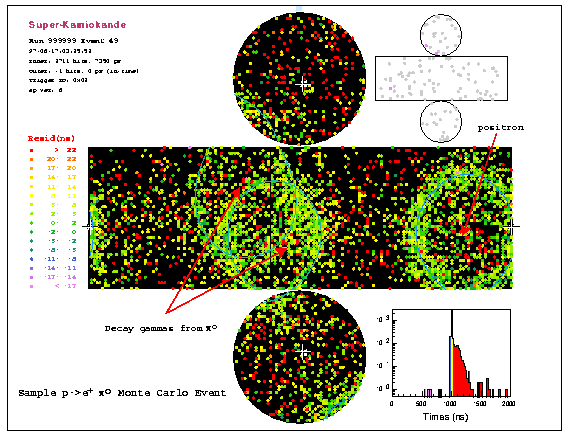
\includegraphics[width=0.9\linewidth]{Figures/epi0_nice_event.png}
    % TODO http://hep.bu.edu/~superk/pdk.html
\end{frame}

\begin{frame}
    References

    \printbibliography
\end{frame}

\end{document}

% vim: spell spelllang=en_us
